% Created 2021-07-13 Tue 19:16
% Intended LaTeX compiler: pdflatex
\documentclass[presentation,aspectratio=169]{beamer}
\usepackage[utf8]{inputenc}
\usepackage[T1]{fontenc}
\usepackage{graphicx}
\usepackage{grffile}
\usepackage{longtable}
\usepackage{wrapfig}
\usepackage{rotating}
\usepackage[normalem]{ulem}
\usepackage{amsmath}
\usepackage{textcomp}
\usepackage{amssymb}
\usepackage{capt-of}
\usepackage{hyperref}
\usepackage{khpreamble}
\usepackage{amssymb}
\usepackage{pgfplotstable}
\DeclareMathOperator{\shift}{q}
\DeclareMathOperator{\diff}{p}
\usetheme{default}
\author{Kjartan Halvorsen}
\date{\today}
\title{Control computarizado - Mínimos cuadrados}
\hypersetup{
 pdfauthor={Kjartan Halvorsen},
 pdftitle={Control computarizado - Mínimos cuadrados},
 pdfkeywords={},
 pdfsubject={},
 pdfcreator={Emacs 26.3 (Org mode 9.4.6)}, 
 pdflang={English}}
\begin{document}

\maketitle

\section{Intro}
\label{sec:org3039ec7}
\begin{frame}[label={sec:orgc3f2bb1}]{Identificación de sistemas}
\end{frame}

\begin{frame}[label={sec:org90d5fe9}]{Un proceso complejo}
\begin{columns}
\begin{column}{0.6\columnwidth}
From Wikipedia "Cyclonic separation"
\end{column}
\begin{column}{0.4\columnwidth}
\begin{center}
\includegraphics[height=1.0\textheight]{../../figures/Vertical-cyclone.jpg}
\end{center}
\end{column}
\end{columns}
\end{frame}

\begin{frame}[label={sec:org6f500c7}]{Identificación de sistemas}
\begin{center}
  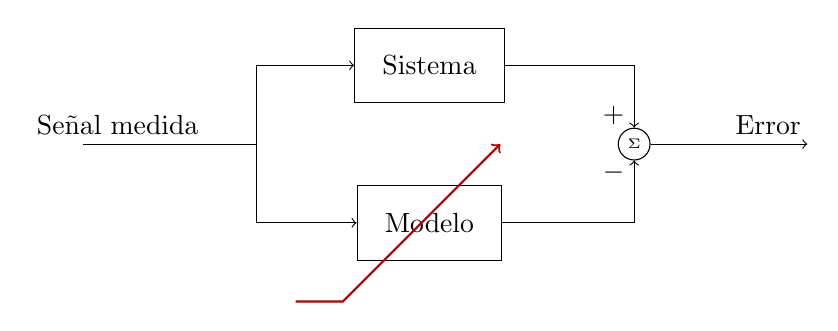
\begin{tikzpicture}[node distance=22mm, block/.style={rectangle, draw, minimum width=15mm, inner sep=10pt}, sumnode/.style={circle, draw, inner sep=2pt},]

    \node[coordinate] (input) {};
    \node[coordinate, right of=input] (copy) {};
    \node[coordinate, right of=copy] (midp) {};
    \node[block, above of=midp, node distance=10mm] (sys)  {Sistema};
    \node[block, below of=midp, node distance=10mm] (mod)  {Modelo};
    \node[sumnode, right of=midp, node distance=26mm] (sum) {\tiny $\Sigma$};
    \node[coordinate, right of=sum, node distance=22mm] (output) {};

    \draw[-] (input) -- node[above, pos=0.2] {Señal medida} (copy);
    \draw[->] (copy) |- node[above] {} (sys);
    \draw[->] (copy) |- node[above] {} (mod);
    \draw[->] (sys) -| node[left, pos=0.9] {$+$} (sum);
    \draw[->] (mod) -| node[left, pos=0.9] {$-$} (sum);
    \draw[->] (sum) -- node[above, near end] {Error} (output);

    \draw[thick, red!70!black, ->] (2.7,-2) -- (3.3,-2) -- (5.3, 0);
  \end{tikzpicture}
\end{center}
\end{frame}

\begin{frame}[label={sec:org0e5956e}]{Ajustando un modelo}
\begin{center}
\includegraphics[height=0.8\textheight]{lsq-example-no-reg}
\end{center}
\end{frame}

\begin{frame}[label={sec:orgd621ef1}]{Ajustando un modelo - regresión lineal}
\begin{columns}
\begin{column}{0.4\columnwidth}
\alert{Objetivo} Dado observaciones \[\mathcal{D} = \{ (x_1,y_1), (x_2, y_2), \ldots, (x_N, y_N)\}\] y 
modelo \(\mathcal{M}: \; y = ax + b  + e\), obtiene los parametros \((a,b)\) que da el modelo que mejor se ajuste a los datos.

El término de ruido, o error, \(e\), incluye errores de modelación y perturbaciones.
\end{column}
\begin{column}{0.6\columnwidth}
\begin{center}
\includegraphics[height=0.6\textheight]{lsq-example}
\end{center}
\end{column}
\end{columns}
\end{frame}


\begin{frame}[label={sec:org378a72b}]{Ajustando un modelo - regresión lineal}
Dado observaciones \(\mathcal{D} = \{ (x_1,y_1), (x_2, y_2), \ldots, (x_N, y_N)\}\) y 
modelo \(\mathcal{M}: \; y = ax + b  + e\). 

\begin{columns}
\begin{column}{0.7\columnwidth}
La predicción es
\[ \hat{y_k} = ax_k + b = \underbrace{\begin{bmatrix} x & 1 \end{bmatrix}}_{\varphi_k^T} \underbrace{\begin{bmatrix} a\\b\end{bmatrix}}_{\theta}\]
y el error de predicción 
\[ \epsilon_k = y_k - \hat{y}_k = y_k - ax_k-b = y - \varphi_k^T\theta.\]

Buscamos parametros \(\theta^T = \begin{bmatrix} a & b \end{bmatrix}\) que minimiza
 la función de pérdida \[J(\theta) =  \sum_{k=1}^N g\big(\epsilon_k\big).\]
\end{column}

\begin{column}{0.3\columnwidth}
\begin{center}
\includegraphics[height=0.4\textheight]{lsq-example}
\end{center}
\end{column}
\end{columns}
\end{frame}


\begin{frame}[label={sec:orge976682}]{Ajustando un modelo - regresión lineal}
Dado observaciones \(\mathcal{D} = \{ (x_1,y_1), (x_2, y_2), \ldots, (x_N, y_N)\}\) y 
modelo \(\mathcal{M}: \; y = ax + b  + e\). 

\begin{columns}
\begin{column}{0.6\columnwidth}
La función de pérdida más común es \alert{mínimos cuadrados}

\begin{align*}
\hat{\theta}_{LS} &= \arg\min J_{LS}(\theta) = \arg\min \sum_{k=1}^N \epsilon_k^2\\
&= \arg\min \sum_{k=1}^N (y_k - \hat{y}_k)^2 
= \arg\min \sum_{k=1}^N (y_k - \varphi_k\T\theta)^2\\ 
&= \arg\min \sum_{k=1}^N (y_k - ax_k - b)^2
\end{align*}
\end{column}

\begin{column}{0.4\columnwidth}
\begin{center}
\includegraphics[height=0.5\textheight]{lsq-example}
\end{center}
\end{column}
\end{columns}
\end{frame}



\begin{frame}[label={sec:org75ca46a}]{El problema con mínimos cuadrados}
\begin{columns}
\begin{column}{0.4\columnwidth}
\begin{align*}
 \text{minimiza} \; &\sum_k g(\epsilon_k)\\
 \text{dónde} \; g(u) &= u^2
\end{align*}
\end{column}

\begin{column}{0.6\columnwidth}
\begin{center}
  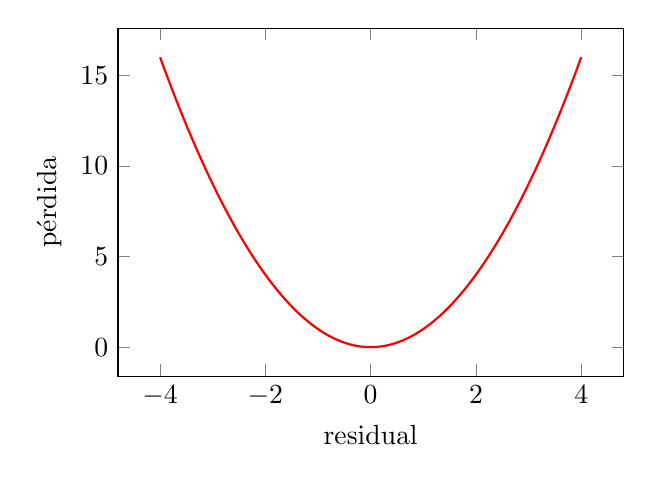
\begin{tikzpicture}
    \begin{axis}[
      width=8cm,
      height=6cm,
      ylabel=pérdida,
      xlabel=residual,
      ]
      \addplot[red, thick, no marks, domain=-4:4, samples=201] {x^2};
    \end{axis}
  \end{tikzpicture}
\end{center}
\end{column}
\end{columns}
\end{frame}

\begin{frame}[label={sec:org240edf5}]{Más robusta: La función de pérdida de Huber}
\begin{columns}
\begin{column}{0.4\columnwidth}
También conocido como \alert{regresión robusta}
\begin{align*}
 \text{minimiza} \; &\sum_k g_{hub}(\epsilon_k)\\
 \text{dónde}\; g_{hub}(u) &= \begin{cases} u^2 & |u| \le M\\ M(2|u|-M) & |u| > M \end{cases}
\end{align*}
\end{column}

\begin{column}{0.6\columnwidth}
\begin{center}
  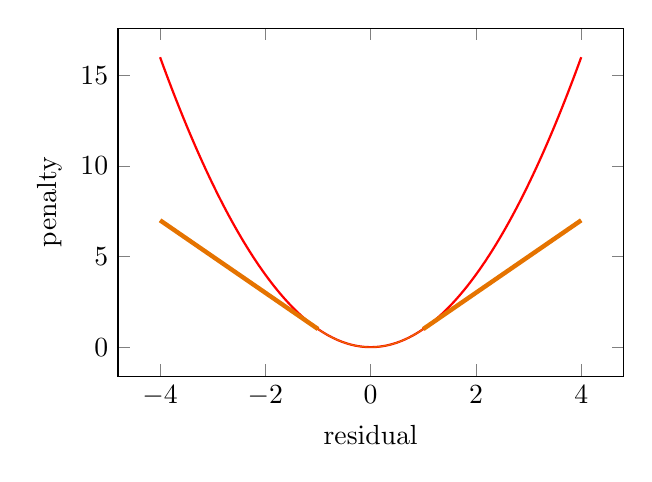
\begin{tikzpicture}
    \begin{axis}[
      width=8cm,
      height=6cm,
      ylabel=penalty,
      xlabel=residual,
      ]
      \addplot[red, thick, no marks, domain=-4:4, samples=201] {x^2};
      \addplot[orange!90!black, ultra thick, no marks, domain=-4:-1, samples=201] {2*abs(x)-1};
      \addplot[orange!90!black, thin, no marks, domain=-1:1, samples=201] {x^2};
      \addplot[orange!90!black, ultra thick, no marks, domain=1:4, samples=201] {2*abs(x)-1};
    \end{axis}
  \end{tikzpicture}
\end{center}
\end{column}
\end{columns}
\end{frame}

\section{AR-model}
\label{sec:org4f000d2}

\begin{frame}[label={sec:org023cc94}]{Ejemplo - Modelo autorregresivo (AR)}
\end{frame}
\begin{frame}[label={sec:org0019461}]{Modelo autorregresivo (AR)}
Dado una secuencia discreta observada \(y(k), \; k=1,2,\ldots,N\), y el modelo autorregresivo
\[ y(k+1) = -ay(k) + e(k+1),\]
dónde \(e(k)\) es una sequencia discreto de ruido blanco.

\alert{Objetivo} Estimar el parametro \(a\).

\begin{enumerate}
\item Forma el predictor de un paso adelante \[\hat{y}_{k+1} = -ay_k=-y_ka = \varphi_{k+1} \theta,\] y el error de predicción \[\epsilon_k = y_k - \hat{y}_k = y_k - \varphi_k \theta\]
\end{enumerate}
\end{frame}


\begin{frame}[label={sec:org27eb1d8}]{Modelo autorregresivo (AR)}
Dado una secuencia discreta observada \(y(k), \; k=1,2,\ldots,N\), y el modelo autorregresivo
\(y(k+1) = -ay(k) + e(k+1),\)
dónde \(e(k)\) es una sequencia discreto de ruido blanco.

\alert{Objetivo} Estimar el parametro \(a\).

\begin{enumerate}
\setcounter{enumi}{1}
\item Reune todas las observaciónes \(y_k\) y predicciones \(\hat{y}_k\) en forma vectoral
\begin{align*}
\epsilon &= \begin{bmatrix} \epsilon_2\\\epsilon_2\\\vdots\\\epsilon_N\end{bmatrix} =  \begin{bmatrix} y_2\\ y_3\\\vdots\\y_N \end{bmatrix} - \begin{bmatrix} \hat{y}_2\\ \hat{y}_3\\\vdots\\\hat{y}_N \end{bmatrix}
 =  \begin{bmatrix} y_2\\ y_3\\\vdots\\y_N \end{bmatrix} - \begin{bmatrix} -y_1 a\\ -y_2 a\\\vdots\\-y_{N-1}^T\theta \end{bmatrix} =  \begin{bmatrix} y_2\\ y_3\\\vdots\\y_N \end{bmatrix} - \begin{bmatrix} \varphi_2^T\theta\\ \varphi_3^T\theta\\\vdots\\\varphi_N^T\theta \end{bmatrix}\\
&= y - \underbrace{\begin{bmatrix}\varphi_1^T\\\varphi_2^T\\\vdots\\\varphi_N^T\end{bmatrix}}_{\Phi}\theta = y - \Phi\theta 
\end{align*}
\end{enumerate}
\end{frame}



\begin{frame}[label={sec:orgda50524}]{Modelo autorregresivo (AR)}
Dado una secuencia discreta observada \(y(k), \; k=1,2,\ldots,N\), y el modelo autorregresivo
\(y(k+1) = -ay(k) + e(k+1),\)
dónde \(e(k)\) es una sequencia discreto de ruido blanco.

\alert{Objetivo} Estimar el parametro \(a\).

\begin{enumerate}
\setcounter{enumi}{2}
\item Obtiene el estimado de mínimos cuadrados 
\begin{align*}
 \theta_{LS} &= (\Phi^T\Phi)^{-1}\Phi^T y\\ &= \left(\begin{bmatrix} -y_1 & -y_2 & \cdots & -y_{N-1}\end{bmatrix}\begin{bmatrix}-y_1\\-y_2\\\vdots\\-y_{N-1}\end{bmatrix}\right)^{-1}\begin{bmatrix} -y_1 & -y_2 & \cdots & -y_{N-1}\end{bmatrix}\begin{bmatrix}y_2\\y_3\\\vdots\\y_N\end{bmatrix}\\
 &= -\frac{\sum_{k=1}^{N-1} y_ky_{k+1}}{\sum_{k=1}^{N-1}y_k^2}
 \end{align*}
\end{enumerate}
\end{frame}


\begin{frame}[label={sec:org87d1346},fragile]{Computación de la solución de mínimos cuadrados}
 Dado error de predicción en forma vectoral para sistema de orden \(n\)
\(\epsilon = y - \Phi\theta\). Forma las \alert{ecuaciones normales}
\begin{align*}
\Phi \theta &= y\\
\begin{bmatrix}\varphi_{n+1}^T\\\varphi_{n+2}^T\\\varphi_{n+3}^T\\\varphi_{n+4}^T\\\vdots\\\varphi_{N}^T\end{bmatrix} \begin{bmatrix}\theta_1\\\theta_2\\\vdots\\\theta_m\end{bmatrix} &= \begin{bmatrix}y_{n+1}\\y_{n+2}\\y{n+3}\\y_{n+4}\\\vdots\\ y_{N}\end{bmatrix}
\end{align*}
Resuelva las ecuaciones normales usando métodos numericamente robustos de algebra lineal, por ejemplo   factorización L-U. En matlab se escribe
\begin{verbatim}
theta_LS = Phi \ y
\end{verbatim}
\end{frame}

\begin{frame}[label={sec:org07df134}]{Ejemplo numerico}
\href{https://mybinder.org/v2/gh/kjartan-at-tec/mr2007-computerized-control/master?filepath=.\%2Fsystem-identification\%2Fnotebooks\%2FAR-example.ipynb}{Mybinder}
\end{frame}





\begin{frame}[label={sec:orgaec78da}]{Modelo autorregresivo (AR) - Ejercicio}
Dado una secuencia discreta observada \(y(k), \; k=1,2,\ldots,N\), y el modelo autorregresivo de segunda orden
\[ y(k+2) = a_1y(k+1) + a_2y(k) + e(k+2),\]
dónde \(e(k)\) es una sequencia discreto de ruido blanco.

\alert{Actividad} Forma las ecuaciones normales \[ \Phi \theta = y\] siguiendo los mismos pasos como en el ejemplo de primer orden.
\end{frame}
\end{document}